\section{Roboterregelung \robo{155}{7}}
\textbf{Regelung Infofluss}
\begin{center}
    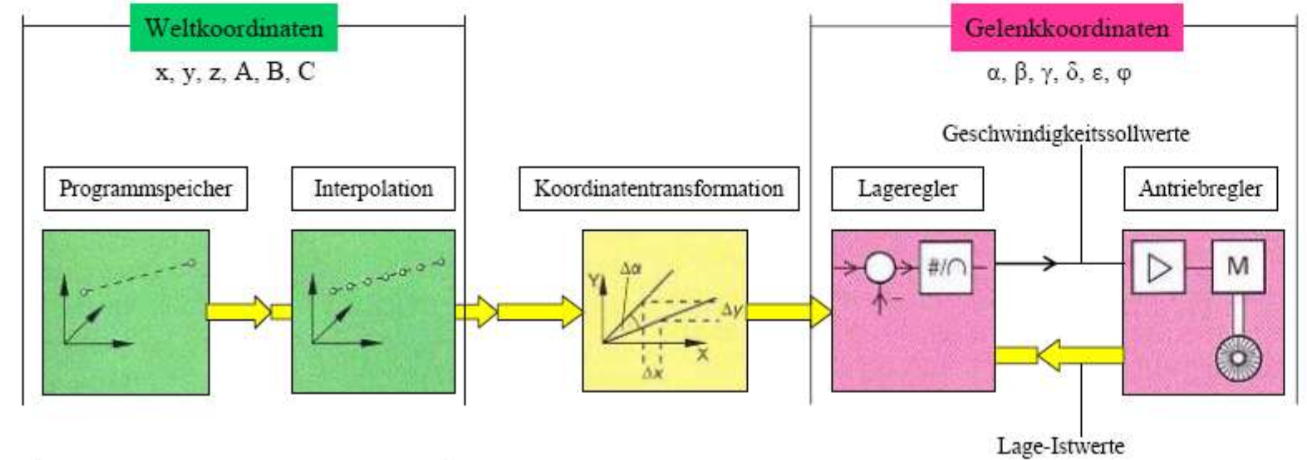
\includegraphics[width=0.9\linewidth]{./bilder/RegelungInfofluss}
\end{center}

\begin{minipage}[t]{0.5\linewidth}
    \textbf{Regelung}
    \begin{itemize}
        \item Lageregelung
        \begin{itemize}
            \item Unabhängig von den Bearbeitungkräften/Momenten
            \item Im Gelenkraum $\rightarrow$ PID oder Modelbasiert
            \item im kartesischen Raum $\rightarrow$ Gelenkbasiert über kinematik oder invers Jacobi
        \end{itemize}
        \item Kraftregelung
        \begin{itemize}
            \item definiert Kräfte/Drehmomente auf die Arbeitsumgebung
        \end{itemize}
        \begin{itemize}
            \item Mischform zwischen Lage und Kraftregelung
        \end{itemize}
        \item hybride Regelung
        \item Interne und externe Roboterregelung
        \item Lineare Regelung
        \item Modelbasierte Regelung
        \item Adaptive Regelung
    \end{itemize}
\end{minipage}
\begin{minipage}[t]{0.5\linewidth}
    \textbf{Steurung}
    \begin{itemize}
        \item Struktur und Komponenten
        \item Ausführungsbeispielö
        \begin{itemize}
            \item ABB, KUKA, Stäuble
        \end{itemize}
    \end{itemize}
\end{minipage}

\begin{minipage}{0.5\linewidth}
    \subsection{Interne/ Externe Regelung}
    \textbf{Interne Regelung/ Gelenkregelung}\newline
    Bearbeitet ausschlieslich Soll- und Messgrössen an den Gelenken.
    Wesentliche Komponente jedes ind. Rob.
    
    \textbf{Externe Regelung}\newline
    Vorallem für fortgeschrittene Robotersteuerungen. Sie ermitteln aus Sensorinformationen und Zielvorgabe der Prog. die notwendigen Bewegungen des Roboters und oder Kräfte des Effektors.
\end{minipage}
\begin{minipage}{0.5\linewidth}
    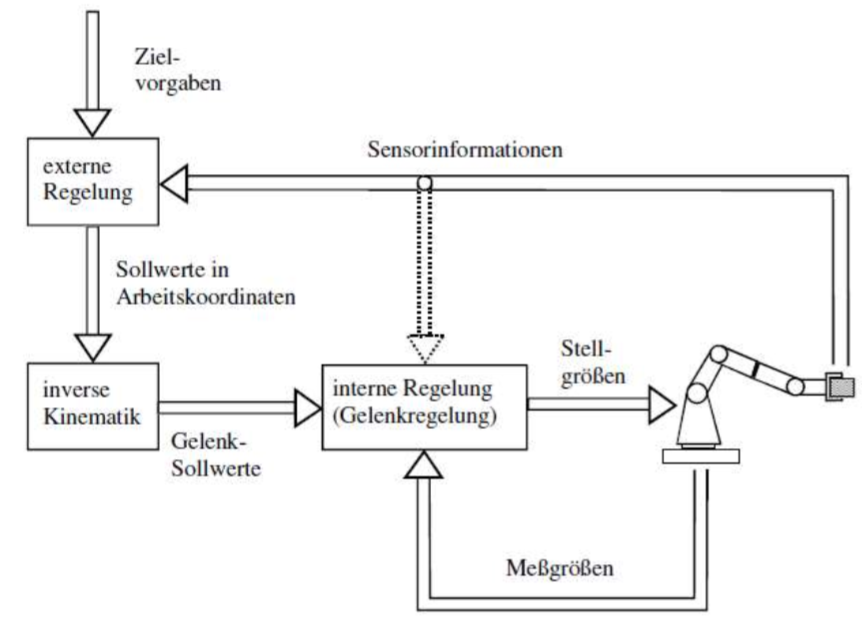
\includegraphics[width=\linewidth]{./bilder/InternExternRegelung}
\end{minipage}

\begin{minipage}{0.5\linewidth}
    \subsection{Lageregelung auf Gelenkebene (intern)}
        \begin{itemize}
            \item[+] Einfache Implementierung
            \item[-] Ungenauigkeit der kart. Pos. TCP
        \end{itemize}
\end{minipage}    
\begin{minipage}{0.5\linewidth}
    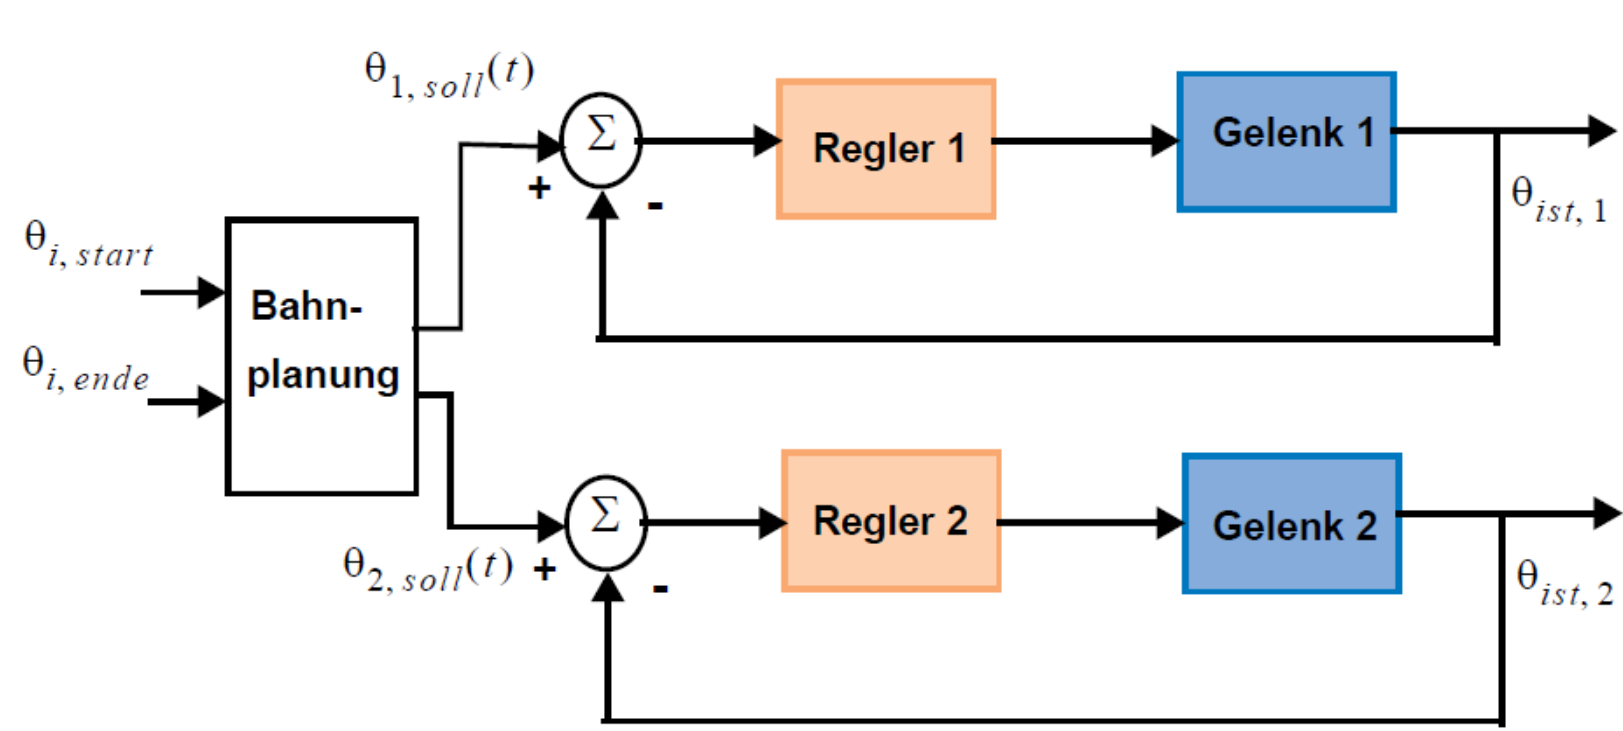
\includegraphics[width=\linewidth]{./bilder/LageregelungGelenk}
\end{minipage}    
\begin{minipage}{0.5\linewidth}
    \subsection{Kartesische Lageregelung (extern)}
    Braucht ein stationäres kartesisches Koord. Sys. (bsp. Kamera) zur erfassung der Position/Orientierung des Effektors. \textbf{X} ist dabei die Orientierung (Vektor des Eulerwinkels) und die Position (Ortsvektor).
    \begin{itemize}
        \item[+] Hohe Positionierungsgenauigketi TCP
        \item[+] Regelungsverhalten wie Schnelligkeit und Dämpfung (ReDuS \robo{164}{7.2.3}) bezgl. TCP
        \item[-] Teueres Erfassungssystem Pos./Orient.
        \item[-] Hohe Rechenleistung nötig
        \item[-] Regelungsprobleme bei Singularität
    \end{itemize}
    
    \robo{195}{7.4.7}
\end{minipage}
\begin{minipage}{0.5\linewidth}
    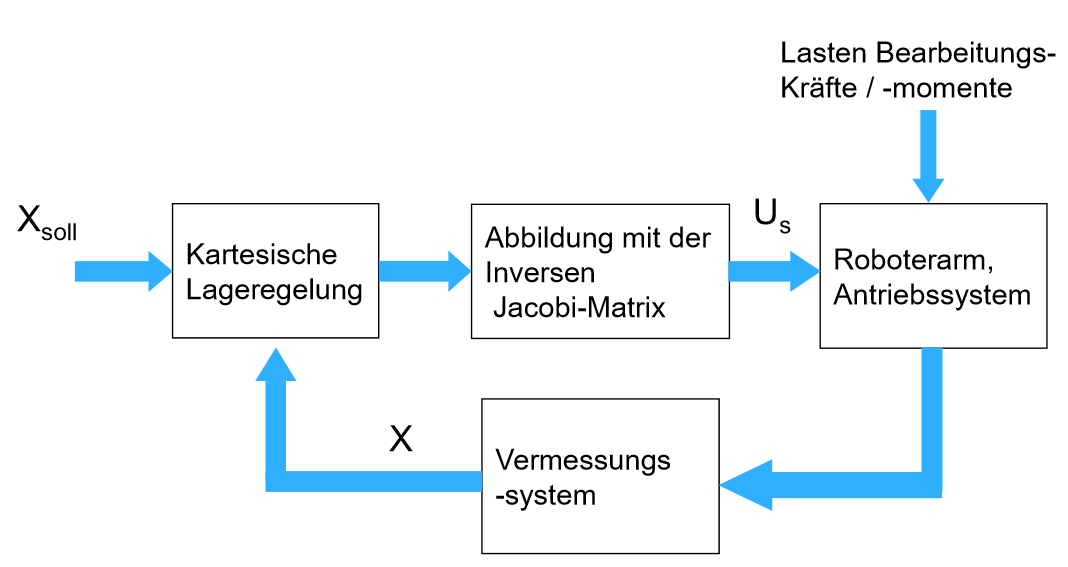
\includegraphics[width=\linewidth]{./bilder/KartLageRegelung}
\end{minipage}

\begin{minipage}{0.5\linewidth}
    \subsection{Kraftregelung \robo{158}{7.1}}
    Kraftregelungen werden eingesetzt, wenn der Roboterarm in Kontakt zu seiner Umgebung tritt unf mit definierten Kräften/Drehmomenten auf eine Umgebung wirken soll.
    Der Kraft/Drehmomentsensor (KMS) ist zwischen Arm und Effektor angebracht.
\end{minipage}
\begin{minipage}{0.5\linewidth}
    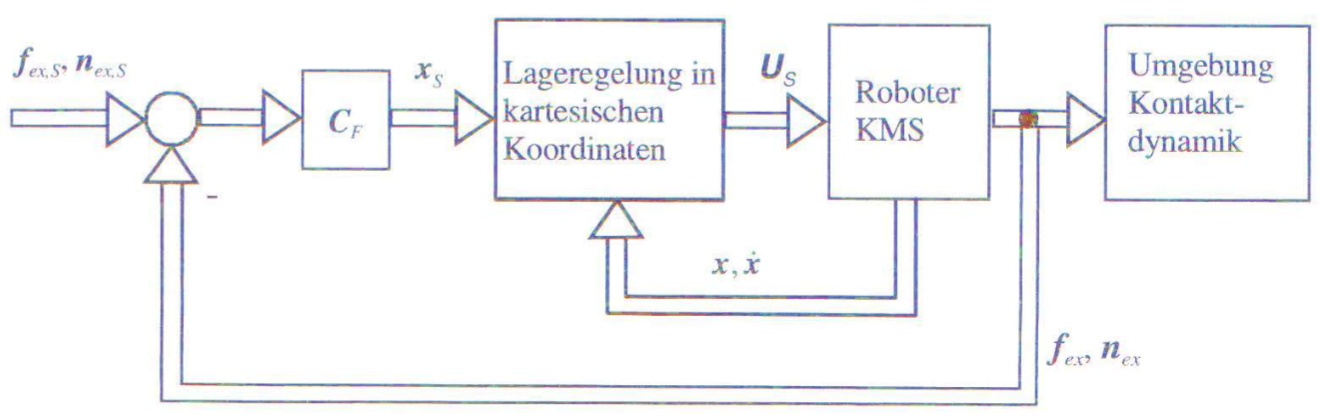
\includegraphics[width=\linewidth]{./bilder/KraftRegelung}
\end{minipage}

\begin{minipage}[b]{0.5\linewidth}
    \subsection{Linearegelung}
    PID \robo{187}{7.4.3}
    \[ \tau_{FB}=K_p\cdot e + K_d\cdot \dot{e} \]
\end{minipage}
\begin{minipage}{0.5\linewidth}
    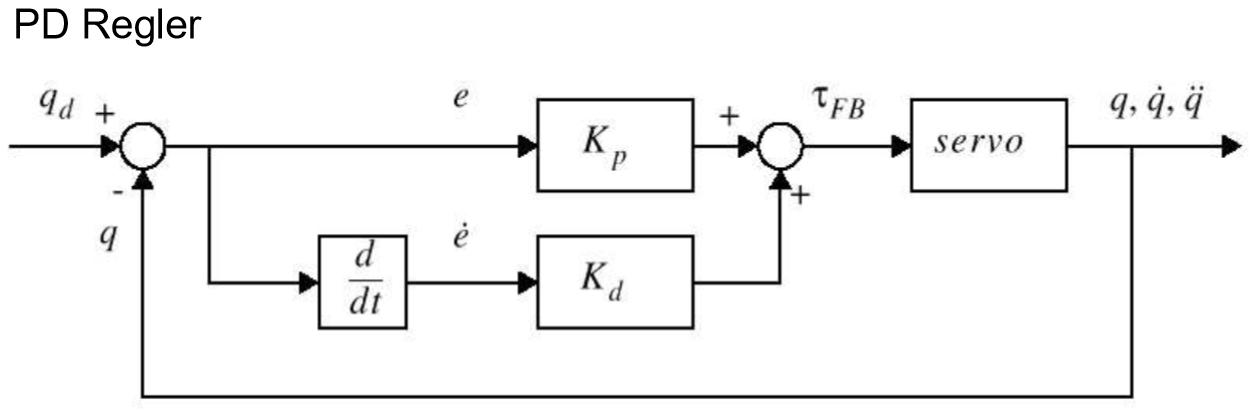
\includegraphics[width=\linewidth]{./bilder/PDRegler}
\end{minipage}


%\begin{minipage}{0.5\linewidth}
%\subsection{Dynamische Gleichung}
%    \[   \tau = M(q)\cdot \ddot{q}+ V(q,\dot{q})+G(q) \]
%    Q = verallgemeinerte Kräfte\newline
%    M = konfigurationsabhängige Massenmatrix\newline
%    V = Vektor nichtlinerer Terme\newline
%    \quad (Centripetal und Coriolis-Beschleunigung)\newline
%    G = Vektor mit Gravitationsterme
%\end{minipage}
\begin{minipage}{0.5\linewidth}
    \subsection{Modellbasierte \robo{182}{7.4}}
    \subsection{Vorsteuerung \robo{182}{7.4.1}}
    Durch die Vorsteuerung wird der Wert der Stellgrösse so vorgegeben, dass die Regelgrösser der Sollgrösse gut folgt. Die Regelung dient nur noch dazu, die Fehler durch ungenaue Vorsteuerung oder Störungen auszugleichen.\newline
    {\small
    + Bessere Dynamik, Regler entlastet, schneller zum Sollwert\newline
    - Hohe Rechenleistung, genaues Modell}
\vspace{-2\baselineskip}
\end{minipage}
\begin{minipage}{0.5\linewidth}
    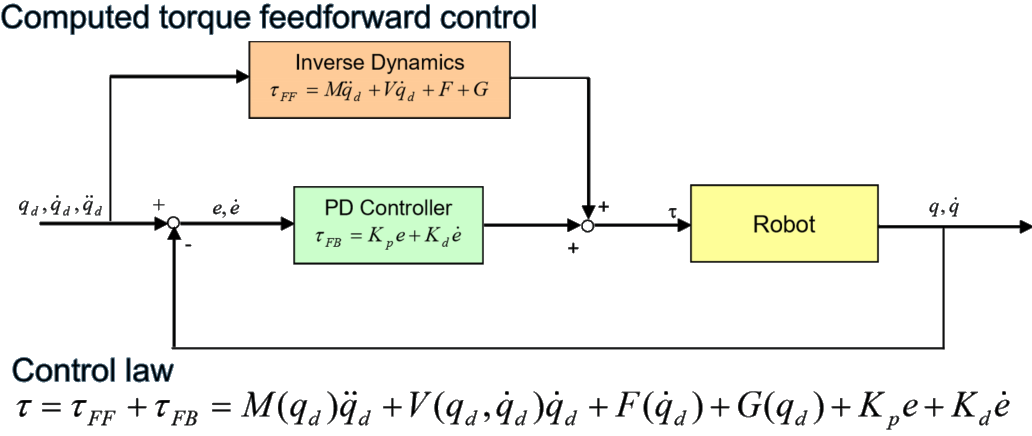
\includegraphics[width=\linewidth]{./bilder/Vorsteuerung}
\end{minipage}

\begin{minipage}{0.5\linewidth}
    \subsection{Adaptive Regelung \robo{179}{7.3}}
    Massnahme zur selbständigen Anpassung eines Reglers auf unterschiedliche Streckenverhältnisse. (Unbekannte Last, Masseträgheitsmoment etc.)
\end{minipage}
\begin{minipage}{0.5\linewidth}
    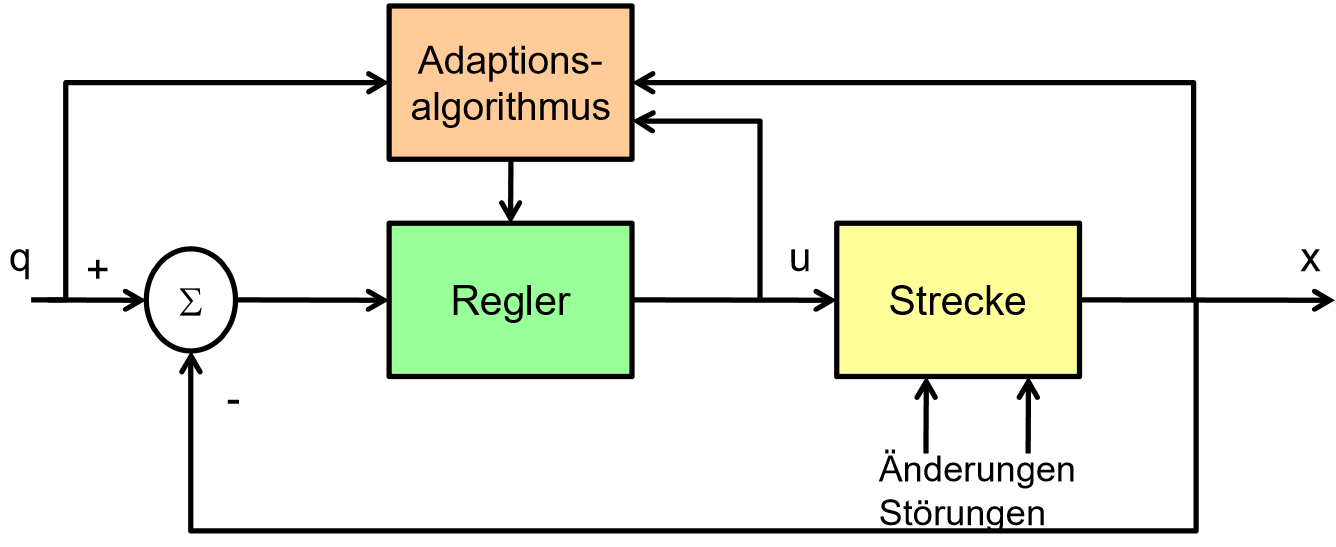
\includegraphics[width=\linewidth]{./bilder/RegAdap}
\end{minipage}

\begin{minipage}{0.5\linewidth}
    \subsection{Drehmomentkontrolle}
    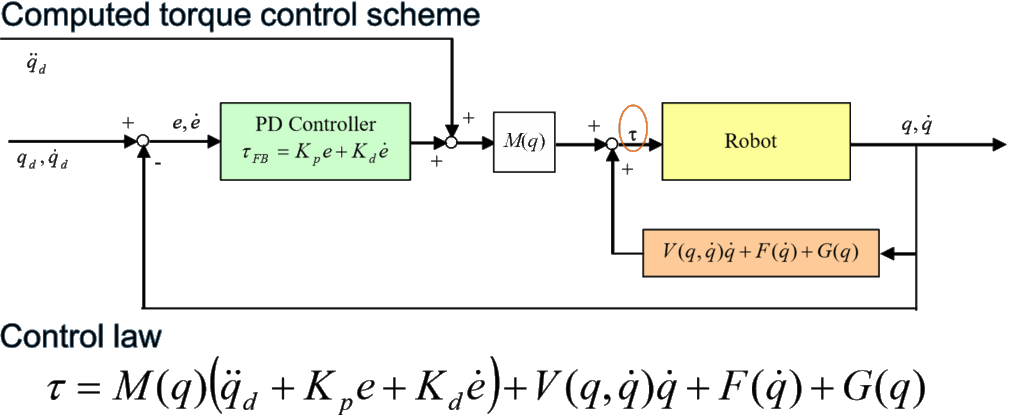
\includegraphics[width=\linewidth]{./bilder/RegMod2}
\end{minipage}
\begin{minipage}{0.5\linewidth}
    \subsection{Nichtlienare Drehmomentkontrolle adaptiv}
    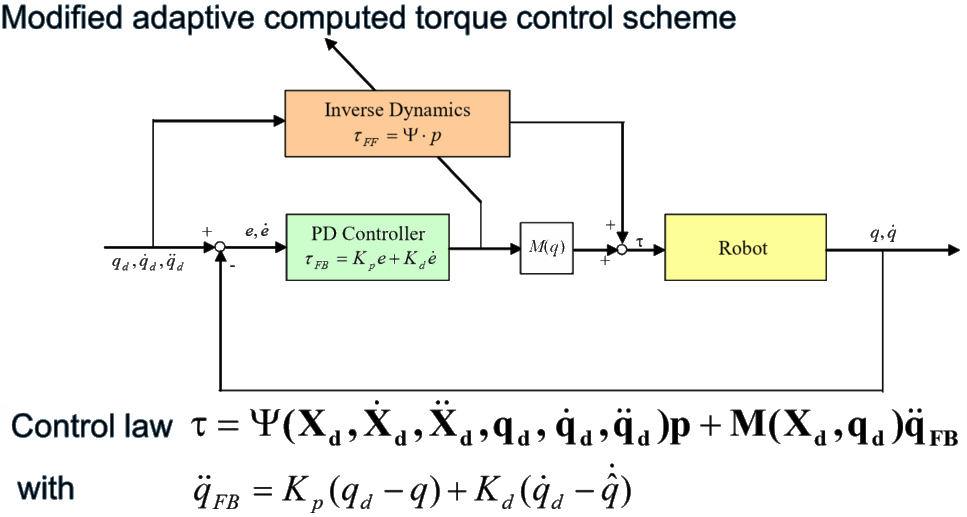
\includegraphics[width=\linewidth]{./bilder/RegModNL}
\end{minipage}

\begin{minipage}[t]{1\linewidth}
    \subsection{Regelung Delta Roboter}
    \raisebox{1\height}{
    \begin{minipage}{0.3\linewidth}
    \begin{itemize}
        \item[]\textbf{Spezifikationen:}
        \item Widerholgenauigkeit v2$\mu$m
        \item Kurze Zykluszeit $\approx$ 3Zyklen/s
    \end{itemize}
\end{minipage}}
    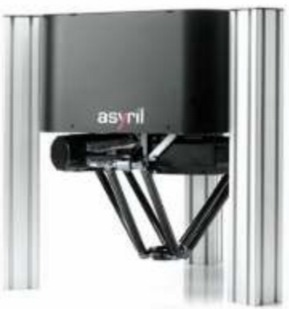
\includegraphics[width=0.17\linewidth]{./bilder/DeltaRob}
    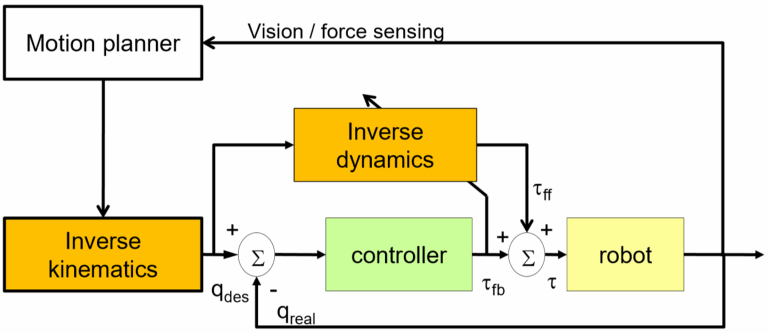
\includegraphics[width=0.5\linewidth]{./bilder/DeltaRobReg}
\end{minipage}
\begin{minipage}[t]{1\linewidth}
    \subsection{Regelung Hexaglide}
    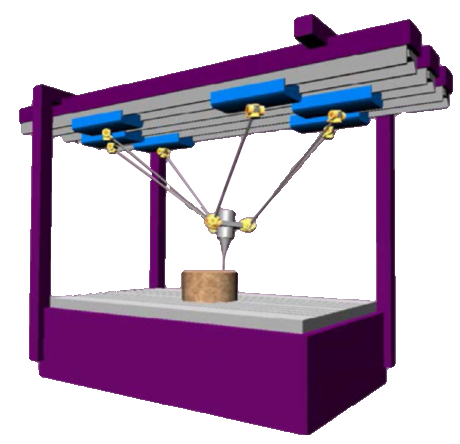
\includegraphics[width=0.2\linewidth]{./bilder/Hexaglide1}
    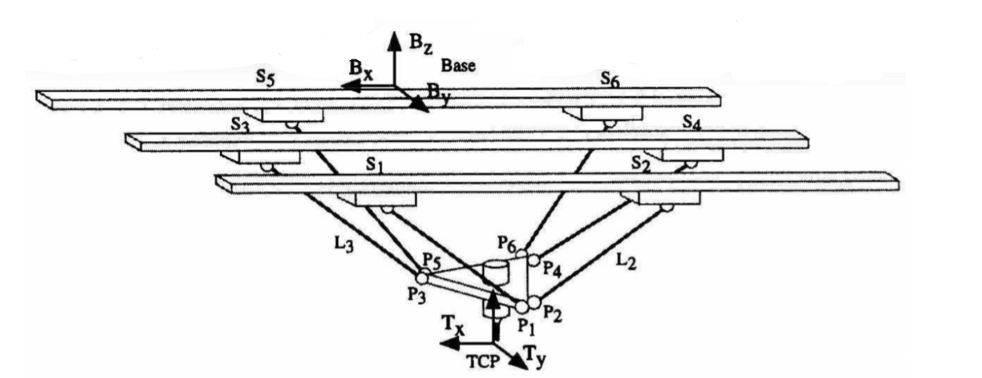
\includegraphics[width=0.3\linewidth]{./bilder/Hexaglide2}
    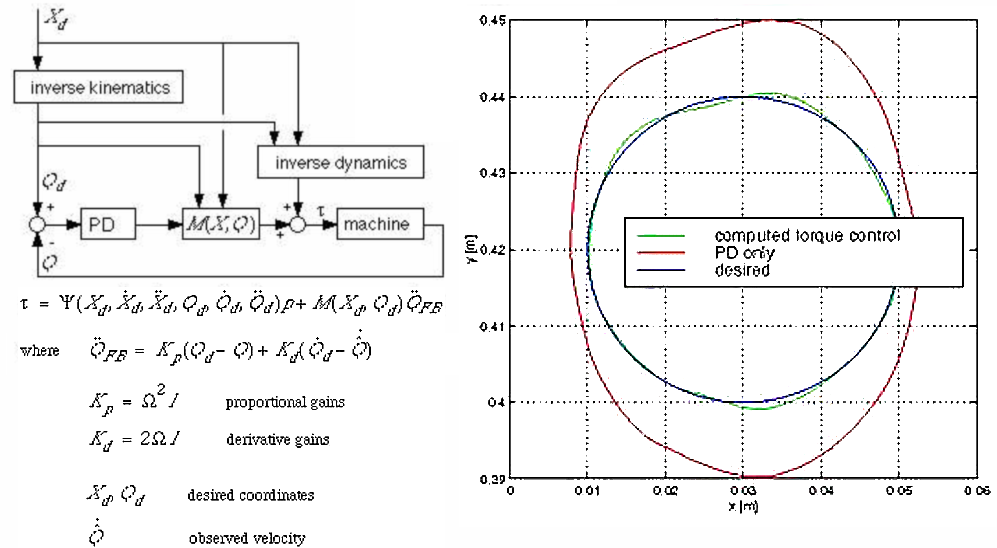
\includegraphics[width=0.5\linewidth]{./bilder/HexaglideReg}
\end{minipage}
\begin{minipage}{0.5\linewidth}
    \subsection{Steuerung ABB}
    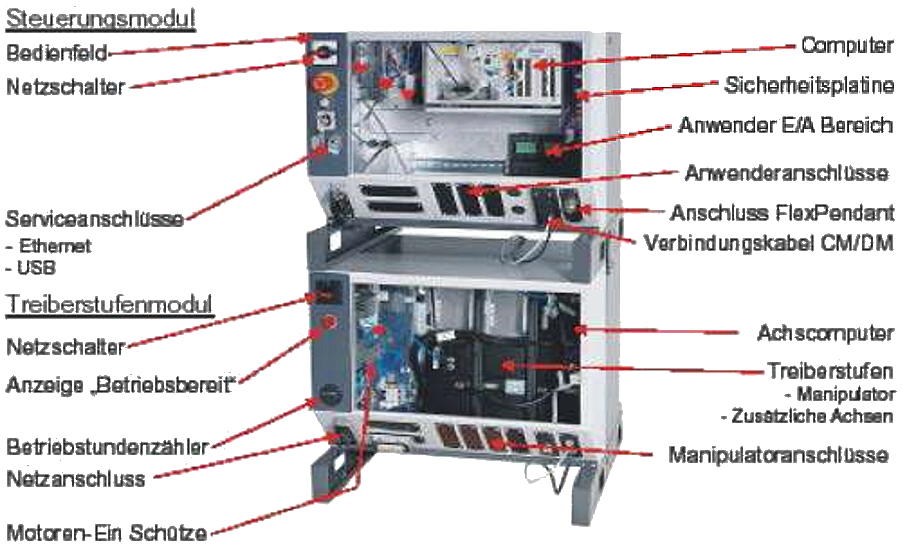
\includegraphics[width=\linewidth]{./bilder/SteuerungABB}
\end{minipage}
\begin{minipage}{0.5\linewidth}
    \subsection{Steuerung Stäubli}
    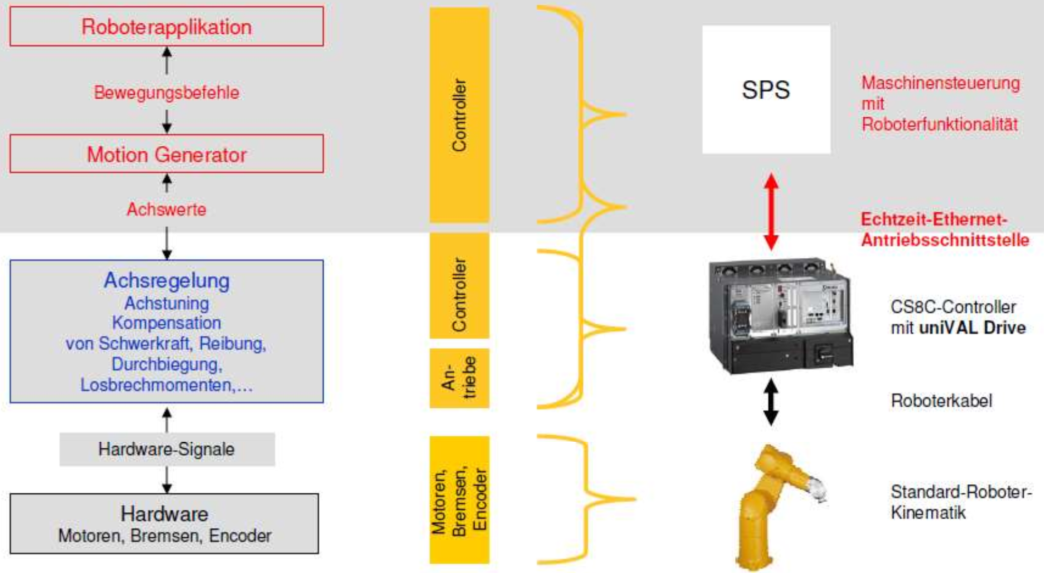
\includegraphics[width=\linewidth]{./bilder/SteuerungStauebli}
\end{minipage}